\documentclass{article}
\usepackage{amssymb} % Required for math symbols
\usepackage{graphicx} % Required for inserting images
\usepackage[hidelinks]{hyperref}
\usepackage{float}

\usepackage[utf8]{inputenc}
\usepackage{amsmath}
\usepackage[a4paper, total={6in, 10in}]{geometry}
\usepackage{listings}
\usepackage{xcolor}

\definecolor{codegray}{rgb}{0.5,0.5,0.5}
\definecolor{codepurple}{rgb}{0.58,0,0.82}
\definecolor{backcolour}{rgb}{0.95,0.95,0.92}

\lstdefinestyle{cppstyle}{
    backgroundcolor=\color{backcolour},   
    commentstyle=\color{codegray}\ttfamily,
    keywordstyle=\color{blue}\bfseries,
numberstyle=\tiny\color{gray},
    stringstyle=\color{codepurple},
    basicstyle=\ttfamily\footnotesize,
    breaklines=true,
    captionpos=b,
    keepspaces=true,
    numbers=left,
    numbersep=5pt,
    showspaces=false,
    showstringspaces=false,
    showtabs=false,
    tabsize=2,
    language=C++
}

\title{Laboratorio 1 - Arduino}
\author{jeremy.matos, luis.gutierrez, plinio.avendano, juan.sara}
\date{Mayo 2025}

\begin{document}

\maketitle

\newpage
\tableofcontents
\newpage

\section{Introducción}

El presente informe documenta el desarrollo del Laboratorio 1 del curso de Internet of Things, cuyo propósito es familiarizar al estudiante con el uso práctico de la plataforma Arduino, facilitando el diseño e implementación de circuitos electrónicos básicos. A través de siete checkpoints progresivos, se exploran conceptos fundamentales como el encendido de LEDs, el uso de resistencias en serie y paralelo, la lectura de entradas digitales mediante botones, la regulación de corriente con potenciómetros, y la simulación de circuitos tanto en Tinkercad como en Falstad. 


\subsection{Objetivo General}

Desarrollar y simular circuitos electrónicos básicos utilizando la plataforma Arduino y herramientas virtuales como Tinkercad y Falstad, aplicando principios fundamentales de electrónica y programación embebida para afianzar competencias prácticas en el diseño e implementación de sistemas digitales.

\subsection{Objetivos Específicos}
\begin{itemize}
    \item Comprender el funcionamiento de componentes electrónicos básicos (LEDs, resistencias, potenciómetros y botones) dentro de circuitos con Arduino.
    \item Simular y analizar circuitos electrónicos en plataformas virtuales como Tinkercad y Falstad.
    \item Implementar lógica de control digital mediante programación en C/C++ en el entorno Arduino IDE.
    \item Representar el comportamiento de sistemas electrónicos mediante diagramas de flujo.
    \item Integrar sensores, actuadores y elementos de control en montajes funcionales como semáforos o secuencias de LEDs.
\end{itemize}

\section{Marco Teórico}
En esta sección se describen los conceptos teóricos fundamentales que sustentan el laboratorio con Arduino. A continuación, se detallan ocho temas clave: desde las características de Arduino y sus pines, pasando por el uso de simuladores y componentes básicos, hasta herramientas de medición y técnicas de diseño relevantes en sistemas embebidos.

\subsection{Descripción general de Arduino (Arduino UNO vs.\ MEGA2560)}
Arduino es una plataforma de hardware y software \textit{open-source} ampliamente utilizada en desarrollo electrónico. Permite que personas sin conocimientos avanzados en electrónica o programación puedan crear prototipos, gracias a la gran cantidad de información y recursos disponibles.\cite{Gonzalez2018} Las placas Arduino incluyen un microcontrolador pre-programado y facilidades de conexión y alimentación, junto con un entorno de desarrollo (IDE) que simplifica la carga de programas (sketches). Existen diversos modelos de placas; entre las más populares están la Arduino Uno y la Arduino Mega 2560, que se diferencian en el microcontrolador utilizado y en sus capacidades de I/O y memoria. La Arduino Uno está basada en el microcontrolador ATmega328P (8 bits a 16~MHz) con 32~KB de memoria flash, 2~KB de SRAM y 14 pines digitales (6 con PWM) más 6 entradas analógicas.\cite{ArduinoUno} Por su parte, la Arduino Mega 2560 incorpora un ATmega2560 (8 bits a 16~MHz) con 256~KB de flash, 8~KB de SRAM, y ofrece 54 pines digitales (15 con PWM) y 16 entradas analógicas.\cite{ArduinoMega} La Mega además dispone de más periféricos integrados, como cuatro puertos serial hardware UART (frente a uno en la Uno). En resumen, la Mega 2560 es adecuada para proyectos de mayor envergadura que requieran más pines de I/O y memoria, mientras que la Uno es suficiente para proyectos básicos y es valorada por su tamaño compacto y bajo costo.

\subsection{Función de los pines digitales, analógicos y especiales}
Las placas Arduino cuentan con pines de propósito general tanto digitales como analógicos, así como pines específicos para funciones particulares. Los \textbf{pines digitales} pueden configurarse como entradas o salidas lógicas (\texttt{HIGH}/\texttt{LOW}), típicamente a niveles TTL de 5~V o 3.3~V según la placa. En modo entrada, pueden leer estados binarios (por ejemplo, detectar si un botón está pulsado o no); en modo salida, pueden conmutar dispositivos (encender/apagar un LED, activar un transistor, etc.).\cite{ArduinoDigitalPins} Algunos pines digitales tienen funciones especiales: por ejemplo, ciertos pines marcan salida PWM (Modulación por Ancho de Pulso) para generar señales analógicas por modulación digital, y los pines $0$ y $1$ suelen estar reservados para comunicación serial (TX/RX). Los \textbf{pines analógicos}, denominados $A0, A1, \dots$, están conectados a un conversor analógico-digital (ADC). Permiten leer señales analógicas continuas (como el voltaje en un sensor variable) y convertirlas a valores numéricos discretos (en Arduino Uno/Mega la resolución es de 10 bits, representando $0$–$5$~V típicamente como $0$–$1023$). Cabe destacar que en los microcontroladores AVR de Arduino, estos pines analógicos también pueden usarse como pines digitales generales si se requiere.\cite{ArduinoAnalogPins} Entre los \textbf{pines especiales} se incluye el pin \texttt{AREF} (referencia analógica externa, usado para fijar un voltaje de referencia distinto al default del ADC), pines de alimentación ($5$V, $3.3$V, GND, Vin), el pin de \texttt{RESET}, y el cabezal ICSP (In-Circuit Serial Programming) que expone líneas SPI y permite reprogramar el microcontrolador a bajo nivel. Adicionalmente, ciertos pines digitales actúan como líneas de comunicación especializadas: por ejemplo, en Arduino Uno los pines analógicos $A4$ y $A5$ se utilizan como SDA y SCL para el bus I\textsuperscript{2}C (TWI), y los pines $10,11,12,13$ soportan SPI (o están duplicados en el conector ICSP). En conjunto, la distribución de pines de Arduino proporciona flexibilidad para interactuar con una variedad de sensores, actuadores y módulos de comunicación.

\subsection{Uso de simuladores Tinkercad y Falstad para circuitos electrónicos}
En el diseño y aprendizaje de circuitos con Arduino resulta muy útil la simulación por software. Dos herramientas destacadas son \textbf{Tinkercad Circuits} y el simulador de circuitos de \textbf{Falstad}. Tinkercad (Autodesk) es una plataforma en línea gratuita que permite armar circuitos electrónicos virtuales e incluso incluir un Arduino virtual programable. Su interfaz gráfica intuitiva posibilita conectar componentes (LEDs, resistencias, pulsadores, sensores, etc.) y escribir código Arduino para simular el comportamiento del circuito en tiempo real. Esta herramienta ha sido aprovechada en entornos educativos técnicos para la enseñanza de electrónica, demostrando facilitar el aprendizaje práctico de los estudiantes en laboratorios virtuales.\cite{Jacob2021} Por su parte, el simulador de Paul Falstad es una aplicación interactiva (basada originalmente en Java, ahora disponible en HTML5) que se centra en la visualización de circuitos analógicos y digitales de forma dinámica. El simulador de Falstad ofrece una representación en tiempo real de corrientes, tensiones y formas de onda, resultando muy útil para comprender fenómenos eléctricos. Estudios comparativos de herramientas de visualización electrónica han mostrado que el simulador de Falstad es altamente efectivo y valorado por los estudiantes, por su simplicidad e interactividad superior frente a otros métodos.\cite{Verbelen2012} En particular, Falstad obtuvo las mejores evaluaciones en criterios de comprensión y entusiasmo del alumno en un entorno de autoaprendizaje.\cite{Verbelen2012} En resumen, Tinkercad permite simular integradamente el circuito y el código Arduino (ideal para prototipos digitales), mientras que Falstad ofrece un enfoque más analógico y formativo en la visualización de principios de electrónica. El uso combinado de ambos simuladores en el laboratorio virtual potencia la comprensión teórica y práctica antes de la implementación física de los circuitos.

\subsection{Principios de funcionamiento de resistencias y potenciómetros (Ley de Ohm)}
Los \textbf{resistores} (o \textit{resistencias} eléctricas) son componentes pasivos cuya función es oponerse al flujo de corriente, siguiendo la relación lineal dada por la Ley de Ohm. Matemáticamente, la ley de Ohm establece que $V = I \cdot R$, es decir, la caída de tensión $V$ en los extremos de una resistencia es proporcional a la corriente $I$ que la atraviesa y a su resistencia $R$.\cite{Alexander2017} Aquí $R$ se mide en ohmios ($\Omega$), $V$ en voltios y $I$ en amperios. Un resistor convierte energía eléctrica en calor (efecto Joule) y se emplea, por ejemplo, para limitar la corriente que pasa por un LED o para definir divisores de tensión. **Potenciómetros**: son resistencias variables de tres terminales que actúan como divisores de tensión ajustables. Un potenciómetro típico consta de una pista resistiva y un contacto deslizante (\textit{wiper}); al girar su eje se modifica la posición del contacto, cambiando la resistencia efectiva entre los terminales. De este modo, si se aplica un voltaje fijo entre los extremos de la pista, el terminal central proporciona un voltaje de salida variable en función de la posición, siguiendo la fórmula del divisor de tensión: $V_{\text{out}} = V_{\text{in}} \cdot \frac{R_2}{R_1+R_2}$ (donde $R_1$ y $R_2$ son las resistencias entre el cursor y cada extremo). Los potenciómetros se utilizan comúnmente para controlar manualmente niveles de audio, brillo de LEDs, ángulos en servomotores, etc. En cualquier circuito con resistencias, se aplica la ley de Ohm localmente para calcular corrientes y tensiones, lo cual es fundamental en el análisis y diseño electrónico básico.\cite{Alexander2017} Por ejemplo, si un LED requiere 10~mA y cae aproximadamente 2~V al conducir, la resistencia en serie con una fuente de 5~V debería ser $R = \frac{5-2}{0.01} = 300~\Omega$ (valor estándar más cercano: 330~$\Omega$) para limitar la corriente de forma segura.\cite{Alexander2017}

\subsection{Uso y estructura del \textit{protoboard} (breadboard) en montaje de circuitos}
El \textbf{protoboard} (del inglés \textit{breadboard}, también llamado \textit{placa de pruebas sin soldadura}) es una base indispensable para armar circuitos electrónicos de forma temporal y reutilizable, sin necesidad de soldaduras. Un protoboard típico consiste en una matriz de agujeros metálicos conectados internamente en filas o columnas. En la zona central, los orificios se agrupan en filas de cinco conectores (llamadas \textit{tiras de bornes}), de modo que insertar dos patillas en la misma fila las conecta eléctricamente. A cada lado de la matriz central suele haber líneas longitudinales denominadas \textit{buses} de alimentación (marcadas con $+$ y $-$), utilizadas para distribuir la tensión de suministro (por ejemplo 5~V y GND) a lo largo de la placa.\cite{Hayes2016} La figura conceptual de un protoboard muestra que está dividido en dos halves por una ranura central (donde típicamente se monta un circuito integrado DIP); las filas a un lado de la ranura están aisladas de las del otro lado, facilitando la inserción de circuitos integrados sin cortocircuitar sus pines opuestos. Para utilizar un protoboard, se conectan los terminales de los componentes en los agujeros de manera que las interconexiones internas formen el circuito deseado. Es importante planificar las conexiones, usando cables de puente (\textit{jumpers}) para enlazar distintos nodos. El protoboard permite modificar el circuito de forma rápida, lo que resulta ideal en la etapa de prototipado y experimentación. Sin embargo, debido a sus conexiones a presión, introduce cierta resistencia de contacto y capacitancia parásita, por lo que no es adecuado para frecuencias muy altas o señales muy sensibles.\cite{Hayes2016} En el contexto del laboratorio con Arduino, el protoboard facilita montar sensores, LEDs, botones y otros componentes alrededor de la placa Arduino, creando un circuito modular y fácilmente modificable para pruebas. Su uso apropiado (manteniendo el orden de cables, evitando confusiones en las filas conectadas y alimentando correctamente los buses) es una habilidad práctica fundamental que los estudiantes deben dominar.\cite{Hayes2016}

\subsection{Instrumentos de medición eléctricos: voltímetro, amperímetro, óhmetro, multímetro}
En el laboratorio electrónico es crucial el manejo de instrumentos de medición para verificar el comportamiento de los circuitos:
\begin{itemize}
  \item \textbf{Voltímetro}: instrumento para medir \textit{diferencias de potencial} (voltaje) entre dos puntos de un circuito.\cite{Bell2013} Un voltímetro ideal tiene una resistencia de entrada muy elevada (teóricamente infinita) para no desviar corriente del circuito bajo medida. Se conecta en \textit{paralelo} al elemento del cual se desea medir la tensión. Los multímetros digitales en modo voltímetro suelen tener impedancias de entrada del orden de megaohmios, minimizando la perturbación del circuito.\cite{Bell2013}
  \item \textbf{Amperímetro}: mide la \textit{corriente eléctrica} que atraviesa un componente o rama del circuito.\cite{Bell2013} Un amperímetro ideal tiene resistencia interna nula, y se conecta en \textit{serie} con el circuito cuyo flujo de corriente se desea medir, de modo que toda la corriente pase a través del instrumento. En la práctica, los amperímetros presentan una pequeña resistencia interna; al usarlos hay que tener cuidado de no sobrepasar su rango, pues una corriente excesiva podría fundir el fusible interno o dañar el equipo.
  \item \textbf{Ohmímetro}: instrumento para medir \textit{resistencias eléctricas}. Funciona inyectando una pequeña corriente de prueba a través del componente y midiendo la caída de tensión resultante, calculando $R = V/I$ internamente.\cite{Bell2013} Se utiliza siempre con el circuito desenergizado (y preferiblemente aislando el componente a medir) para evitar lecturas erróneas. En multímetros digitales, el modo óhmetro suele tener varios rangos de medida y puede emitir un aviso sonoro de continuidad cuando la resistencia es muy baja (indicando conexión directa).
  \item \textbf{Multímetro}: combina las funciones de voltímetro, amperímetro y óhmetro en un solo equipo portátil.\cite{Bell2013} Los multímetros modernos, generalmente digitales, poseen un conmutador para seleccionar la magnitud a medir y el rango adecuado. Suelen incluir también funciones adicionales como medición de capacitancia, frecuencia, prueba de diodos y continuidad. En el laboratorio con Arduino, el multímetro es una herramienta esencial para diagnosticar el circuito: permite verificar, por ejemplo, que el voltaje de alimentación es el correcto, medir la corriente que consume un dispositivo o comprobar el valor de una resistencia antes de integrarla en el diseño.
\end{itemize}
Es fundamental comprender la correcta conexión de cada instrumento: un voltímetro mal colocado (en serie) o un amperímetro en paralelo pueden alterar el circuito e incluso dañarse. Por ello, las prácticas de laboratorio enfatizan el uso apropiado del multímetro en sus diferentes modos, siguiendo los principios eléctricos básicos.\cite{Bell2013}

\subsection{Funcionamiento electrónico de botones y LEDs}
En los sistemas con Arduino es común la interacción mediante \textbf{LEDs} (como salidas visuales) y \textbf{pulsadores} o botones (como entradas manuales). Comprender su funcionamiento electrónico es crucial para un diseño correcto:
\begin{itemize}
  \item \textbf{LED (Diodo Emisor de Luz)}: Es un diodo semiconductor que emite luz al polarizarse en directo. Electrónicamente, el LED permite el paso de corriente en un sentido (ánodo a cátodo) a partir de cierta tensión umbral (aprox. 1.8–2.2~V para LEDs rojos, hasta ~3 V para azules/blancos). Para operar un LED con seguridad, **siempre** se coloca una resistencia en serie que limite la corriente a un nivel seguro (p.ej. $10$–$20$~mA típicamente).\cite{Horowitz2015} Sin esta resistencia, el LED se comportaría casi como un cortocircuito una vez superada la tensión de umbral, pudiendo quemarse por exceso de corriente. En un circuito con Arduino, un pin digital configurado como salida puede excitar un LED: por convención se suele conectar el ánodo del LED al pin Arduino (vía resistencia en serie) y el cátodo a masa (LED encendido con salida HIGH), o alternativamente ánodo a +5V, cátodo al pin (LED encendido con LOW, usando la resistencia para limitar corriente al ir a GND). El LED integrado en la placa Arduino (usualmente conectado al pin 13 en la Uno) facilita pruebas básicas de parpadeo. Cabe destacar que el brillo percibido del LED puede controlarse variando la corriente o mediante PWM (parpadeo rápido), técnica implementada por Arduino al usar \texttt{analogWrite} sobre pines PWM.
  \item \textbf{Pulsador (Botón)}: Es un interruptor mecánico momentáneo que, al ser presionado, cierra un circuito. Electrónicamente, un pulsador se modela como un contacto que puede conectar dos nodos (por ejemplo, unir un pin de entrada digital de Arduino a 0~V cuando se presiona). Un aspecto importante es que cuando el botón está \textit{libre} (no presionado), la entrada del microcontrolador no debe quedar \textit{flotante} (indefinida), ya que recogería ruido eléctrico. Para evitarlo se usan \textbf{resistencias de polarización} (pull-up o pull-down). La práctica común con Arduino es habilitar la resistencia \textit{pull-up} interna del microcontrolador en el pin de entrada, la cual conecta débilmente el pin a +5~V. Así, cuando el pulsador está abierto el pin lee HIGH (5~V a través de la resistencia), y cuando el pulsador se cierra a masa, el pin lee LOW (0~V).\cite{Horowitz2015} De esta forma se define un estado estable en ausencia de pulsación. Alternativamente, se puede usar un esquema inverso con resistencia pull-down a GND y conectar el pulsador a +5~V, pero Arduino facilita más la primera opción mediante \texttt{pinMode(pin, INPUT\_PULLUP)}. Otro fenómeno a considerar es el \textbf{rebote} (\textit{bouncing}): los contactos metálicos del pulsador vibran brevemente al hacer o romper contacto, provocando que la señal de entrada pueda fluctuar entre 0 y 1 durante unos milisegundos. Este rebote puede inducir lecturas erróneas (p.ej., múltiples detecciones de un solo pulsación). Para mitigar el efecto, se implementa \textbf{debounce}, ya sea por hardware (filtrado RC, esquemas Schmitt trigger) o por software (ignorando cambios muy rápidos en el estado durante un intervalo corto de tiempo).\cite{Horowitz2015} En los programas Arduino típicos, se incorpora un retraso o se verifica que el estado se mantenga estable cierta cantidad de milisegundos antes de confirmar una pulsación. En resumen, un pulsador proporciona una interfaz simple para entrada digital, pero requiere un acondicionamiento básico (resistencia de pull-up/pull-down y manejo de rebote) para integrarse fiablemente en el sistema.
\end{itemize}

\subsection{Diagramas de flujo como herramienta en programación y diseño embebido}
Los \textbf{diagramas de flujo} son representaciones gráficas de algoritmos o procesos, empleadas como una valiosa herramienta de planificación y diseño en sistemas embebidos. Un diagrama de flujo utiliza símbolos normalizados (óvalos para inicio/fin, rectángulos para procesos/instrucciones, rombos para decisiones lógicas, paralelogramos para entradas/salidas, flechas para flujo de secuencia, etc.) para describir de forma visual los pasos que seguirá un programa o sistema.\cite{Tarsini2024} En el contexto de la programación de microcontroladores (como Arduino), los diagramas de flujo permiten bosquejar la lógica antes de codificarla en C/C++. Por ejemplo, al desarrollar el firmware de un Arduino que lee un sensor y controla un actuador, un diagrama de flujo ayuda a clarificar las condiciones (p.ej. \textit{“si la temperatura supera X, entonces encender ventilador”}) y el orden de las acciones (lecturas, cálculos, decisiones, bucles) de manera intuitiva. Esto facilita la detección de posibles casos no contemplados o la simplificación de la secuencia de operaciones.\cite{Tarsini2024} Además, sirven como documentación para que otros ingenieros comprendan rápidamente el funcionamiento lógico del sistema sin leer código fuente. Un diagrama de flujo bien elaborado muestra caminos alternativos (ramas condicionales) y bucles (iteraciones) de un algoritmo embebido. Por ejemplo, en un sistema de semáforo controlado por Arduino, el diagrama de flujo delineará los estados (verde, amarillo, rojo), el temporizador para cambios de estado, y las transiciones entre estados basadas en tiempo o sensores. Herramientas de desarrollo moderno pueden traducir diagramas de flujo en código (lenguajes de programación visual), pero incluso dibujados a mano, son valiosos para el \textit{debugging} lógico. En suma, el uso de diagramas de flujo en el diseño de sistemas embebidos proporciona una visión estructurada de la solución antes de implementarla en código, mejorando la claridad y reduciendo errores lógicos durante el desarrollo.\cite{Tarsini2024} Es una práctica recomendada, sobre todo en etapas educativas, para fomentar el pensamiento algorítmico y la comunicación de la estructura de un programa.
\section{Estado del Arte}

La ense\~nanza de sistemas embebidos e Internet de las Cosas (IoT) conlleva retos importantes, como la necesidad de equipamiento f\'isico costoso y la complejidad de los conceptos multidisciplinares involucrados. En este contexto, los simuladores electrónicos y plataformas de prototipado virtual han emergido como herramientas did\'acticas fundamentales para complementar la teor\'ia con pr\'acticas accesibles y seguras\cite{Albiter2019, Contreras2010}. Diversos estudios se\~aalan que el uso de simuladores facilita la comprensión de los principios de electrónica, al permitir que los estudiantes experimenten de forma interactiva con circuitos y código sin riesgo para los equipos f\'isicos. Por ejemplo, Albiter et al. \cite{Albiter2019} destacan la importancia del software de simulación en la comprensión del funcionamiento de componentes electrónicos, evidenciando que las herramientas digitales pueden mejorar el aprendizaje de conceptos abstractos. Asimismo, Contreras et al. \cite{Contreras2010} tempranamente identificaron que los entornos virtuales propician la transferencia de conocimiento en \'areas tecnológicas. M\'as recientemente, un meta-an\'alisis confirmó que los laboratorios virtuales tienen un impacto positivo significativo en el rendimiento académico y la motivación de los alumnos en disciplinas STEM\cite{Zaturrahmi2020}. Esto refuerza el valor pedagógico de las simulaciones en educación, especialmente frente a escenarios de ense\~aanza remota o h\'ibrida donde el acceso a laboratorios f\'isicos puede ser limitado.
\\\\
Dentro de estas herramientas, Tinkercad (plataforma web de Autodesk) ha ganado notable protagonismo en el \'ambito educativo. Originalmente concebida para dise\~ao 3D, Tinkercad incluye un entorno de simulación de circuitos y Arduino que resulta altamente accesible (gratuito y basado en navegador) y f\'acil de usar para estudiantes novatos. Su empleo en cursos de electrónica y programación se ha asociado con mejoras en diversas competencias estudiantiles. Eryilmaz y Deniz \cite{Eryilmaz2021} reportan que la incorporación de Tinkercad en actividades de programación con Arduino mejoró significativamente las habilidades de pensamiento computacional de los alumnos, adem\'as de influir positivamente en sus actitudes hacia la materia. De igual forma, Juanda y Khairullah \cite{Juanda2020} hallaron que este software optimizó el proceso de ense\~aanza-aprendizaje en una asignatura de Electrónica y Microprocesadores, permitiendo a los estudiantes visualizar y experimentar con conceptos abstractos de forma interactiva, lo que facilitó su comprensión. En contextos de educación secundaria, Tinkercad también ha demostrado ser una herramienta efectiva para lograr aprendizajes significativos: según Chiluisa et al. \cite{Chiluisa2022}, el uso estratégico de este simulador contribuyó a una mejor comprensión de los circuitos eléctricos, evidenciada por incrementos en el rendimiento estudiantil después de su implementación. Cabe destacar que durante la pandemia de COVID-19, Tinkercad se utilizó como alternativa para la instrucción pr\'actica a distancia; Villalba et al. \cite{Villalba2021} documentan cómo estudiantes pudieron aprender conceptos b\'asicos de electrónica desde casa usando esta plataforma, manteniendo la continuidad educativa a pesar de las restricciones de acceso a laboratorios f\'isicos. Estos hallazgos consolidan a Tinkercad como una herramienta vers\'atil en la ense\~aanza de electrónica, robótica e IoT, al posibilitar un entrenamiento pr\'actico virtual que complementa la experimentación con hardware real.
\\\\
Adem\'as de Tinkercad, existen simuladores de circuitos en l\'inea como el desarrollado por Paul Falstad (conocido simplemente como Falstad Circuit Simulator, actualmente disponible como CircuitJS). Este entorno ofrece una simulación interactiva en tiempo real de circuitos analógicos y digitales a través del navegador, caracteriz\'andose por su sencillez y naturaleza visual. Aunque Falstad no simula microcontroladores, es ampliamente empleado para la ense\~aanza de fundamentos de electrónica, ya que permite visualizar instant\'aneamente fenómenos como la distribución de corrientes, ca\'idas de tensión en componentes y formas de onda, facilitando la conexión entre la teor\'ia y la pr\'actica en circuitos b\'asicos. Su valor pedagógico reside en la retroalimentación inmediata: los estudiantes pueden modificar par\'ametros de un circuito (por ejemplo, cambiar un valor de resistencia o capacitor) y observar al instante los efectos, lo que refuerza su comprensión de conceptos abstractos y les permite aprender por indagación. Solórzano y Estrella \cite{Solorzano2024} resaltan que este tipo de simulaciones interactivas, integradas con estrategias did\'acticas lúdicas, incrementan significativamente la motivación y el rendimiento en cursos de circuitos eléctricos, al permitir a los alumnos manipular modelos virtuales de los sistemas estudiados. En suma, herramientas ligeras como Falstad complementan la formación en electrónica al posibilitar una experimentación virtual r\'apida y accesible. Esto prepara a los estudiantes para afrontar circuitos m\'as complejos y sienta bases sólidas antes de migrar a plataformas de simulación m\'as avanzadas o a montajes con hardware real.
\\\\
Por otra parte, Arduino se ha consolidado como una plataforma central en la ense\~aanza de sistemas embebidos e IoT. Desde su introducción en 2005, el ecosistema Arduino (hardware de bajo costo y software libre) se ha adoptado extensamente en educación debido a su facilidad de uso y a la gran comunidad de desarrolladores que lo respalda. En entornos académicos, Arduino permite que estudiantes de pregrado e incluso nivel medio superior construyan prototipos funcionales con sensores, actuadores y módulos de comunicación, materializando conceptos abstractos de programación y electrónica en proyectos tangibles\cite{Vidal2019}. Numerosos trabajos reportan resultados positivos al integrar Arduino en la curr\'icula. Por ejemplo, Tupac et al. \cite{Tupac2021} describen los beneficios de utilizar proyectos con Arduino en un curso introductorio de programación: se observó un mayor involucramiento de los alumnos y una mejor comprensión de la interacción hardware-software, al aplicar la teor\'ia de forma pr\'actica en la resolución de problemas reales. De modo similar, Vidal et al. \cite{Vidal2019} relatan experiencias exitosas en las que estudiantes desarrollaron soluciones tecnológicas basadas en Arduino, promoviendo el aprendizaje activo y el desarrollo de competencias pr\'acticas en electrónica y programación. Arduino, por tanto, no solo acerca a los estudiantes a los principios de los sistemas embebidos, sino que también los introduce al mundo IoT mediante proyectos donde, por ejemplo, conectan sus dispositivos a internet o implementan redes de sensores.
\\\\
En la formación orientada al IoT, el uso de Arduino se ve potenciado al combinarlo con simuladores virtuales. Estudios en contextos de IoT educativo muestran que emplear previamente una simulación como Tinkercad para diseñar y probar circuitos con Arduino proporciona a los alumnos una base sólida antes de la experimentación física \cite{Lozoya2022}. Lozoya-Pérez et al. \cite{Lozoya2022} documentan que en una materia de laboratorio IoT, la incorporación de simuladores (Tinkercad, entre otros) facilitó el proceso de enseñanza-aprendizaje, evidenciado por un mejor desempeño de los estudiantes en las prácticas. En dicho estudio, se recomienda utilizar la simulación previa en conjunto con la práctica física, ya que el estudiante logra una mayor comprensión de los resultados de aprendizaje al ensayar primero en un entorno virtual seguro y luego trasladar ese conocimiento al hardware real. Esta aproximación mixta (simulación + experimentación) optimiza el tiempo de laboratorio y reduce errores de montaje, enriqueciendo la experiencia formativa. Por ejemplo, Markushevich (2020)\cite{markushevich2020} documenta el uso de Tinkercad en la enseñanza a distancia de robótica con Arduino Uno, señalando que la simulación virtual resulta eficaz cuando no se dispone de componentes físicos. Del mismo modo, Vibhute (2022) destaca que Tinkercad facilita la comprensión de conceptos al ofrecer una experiencia práctica simulada muy similar a la de un laboratorio físico, mejorando el aprendizaje en electrónica y programación \cite{vibhute2022}. Navas-González (2022) también describe cómo los estudiantes utilizan Tinkercad para simular proyectos en instrumentación biomédica antes de realizarlos físicamente, lo cual optimiza la preparación para actividades prácticas \cite{navas2022}. Asimismo, Abburi et al. (2021) \cite{abburi2021} señalan que Tinkercad, como laboratorio virtual, mejora la participación de los estudiantes y les permite practicar habilidades clave de manera segura, especialmente útil durante situaciones de educación remota. Finalmente, Tupac-Yupanqui et al. (2021) \cite{tupac2021} muestran que el uso de Arduino y Tinkercad en cursos de primer año tuvo un impacto positivo en el desarrollo de competencias de programación, incluso en modalidad virtual, comparado con cohortes anteriores. La literatura actual, por tanto, respalda la integración de herramientas como Tinkercad, simuladores tipo Falstad y plataformas Arduino en la educación tecnológica, ya que potencian el aprendizaje al ofrecer entornos prácticos complementarios que mejoran la comprensión y preparan a los alumnos para los desafíos de la Ingeniería en la era digital.

\section{Metodolog\'ia}

En esta sección se describir\'a el desarrollo de cada una de las experiencias del laboratorio.

\subsection{Checkpoint 1: Creación de un circuito b\'asico}

Este ejercicio introductorio propone la implementación de un circuito b\'asico utilizando un diodo LED y una resistencia (Figura \ref{fig:circuito_basico}). 
% El objetivo es observar el funcionamiento del diodo LED y medir la ca\'ida de tensión en sus terminales.

\begin{figure}[H]
    \centering
    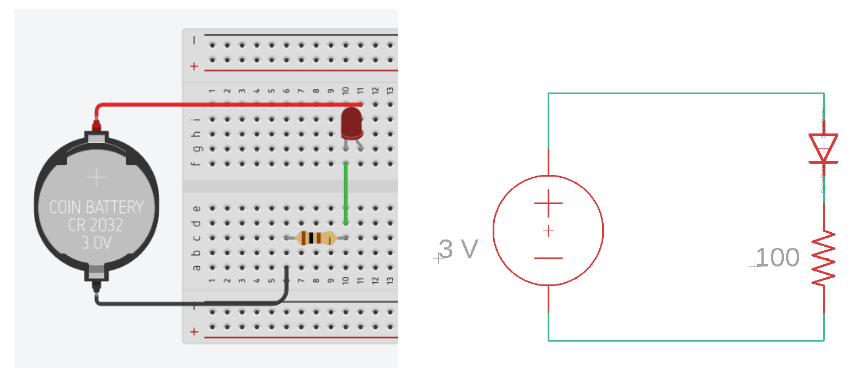
\includegraphics[width=0.85\textwidth]{./img/ckpt_1_0.png}
    \caption{Circuito b\'asico con un diodo LED y una resistencia.}
    \label{fig:circuito_basico}
\end{figure}

\begin{enumerate}
    \item \textbf{Descripción del circuito:} \\
    El circuito est\'a compuesto por una bater\'ia tipo moneda de 3V, un diodo LED conectado en serie y una resistencia de 100~$\Omega$ para limitar el paso de corriente. Luego, se conectar\'a un volt\'imetro en paralelo con el LED para medir la ca\'ida de tensión y un amper\'imetro después de la resistencia para medir la corriente que atraviesa el circuito (Figura \ref{fig:caida_tension}).

    \item \textbf{¿Cu\'al es el valor de la ca\'ida de tensión en los terminales del diodo LED?} \\
    De acuerdo a la Figura \ref{fig:caida_tension}, la ca\'ida de tensión en los terminales del diodo LED es de \textbf{1.98 V}.

    \item \textbf{¿Cu\'al es el valor de corriente obtenido en el circuito?} \\
    El valor de corriente medido con el amper\'imetro fue de \textbf{9.30 mA} (miliamperios) (Figura \ref{fig:caida_tension}).

    \item \textbf{¿Cu\'al es la potencia consumida por el diodo LED?} \\
    Usando la fórmula $P = V \times I$, donde $V = 1.98$ V y $I = 9.3$ mA, se obtiene una potencia de aproximadamente \textbf{18.414 mW}.
\end{enumerate}

\begin{figure}[H]
    \centering
    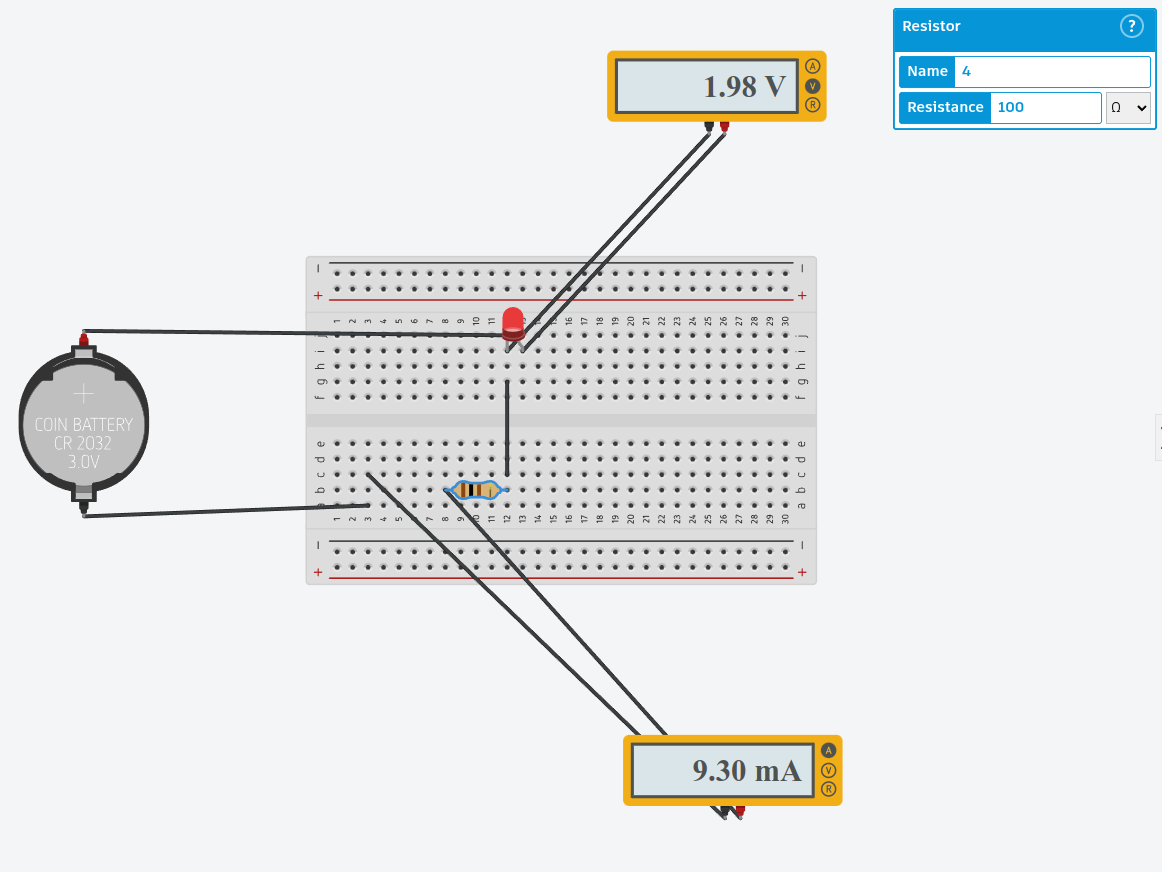
\includegraphics[width=0.85\textwidth]{./img/ckpt_1_1.png}
    \caption{Medida de ca\'ida de tensión.}
    \label{fig:caida_tension}
\end{figure}

\subsection{Checkpoint 2: Conexión de resistencias en serie y paralelo}

Similar al ejercicio anterior, se propone la implementación de 2 circuitos con resistencias en serie y paralelo.

\subsubsection{Circuito 1}

El primer circuito consiste en conectar un diodo LED simple a una resistencia como se ve en Figura \ref{fig:resistencia_serie}. Mientras que el segundo propone conectar 2 resistencias en paralelo, como se ve en la Figura \ref{fig:resistencia_paralelo}. 

\begin{figure}[H]
    \centering
    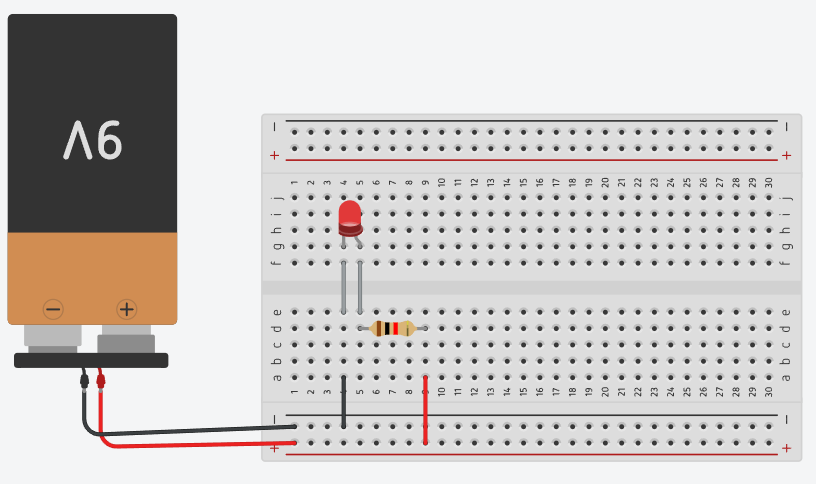
\includegraphics[width=0.5\textwidth]{./img/ckpt_2_1.png}
    \caption{Resistencia en serie}
    \label{fig:resistencia_serie}
\end{figure}


\begin{figure}[H]
    \centering
    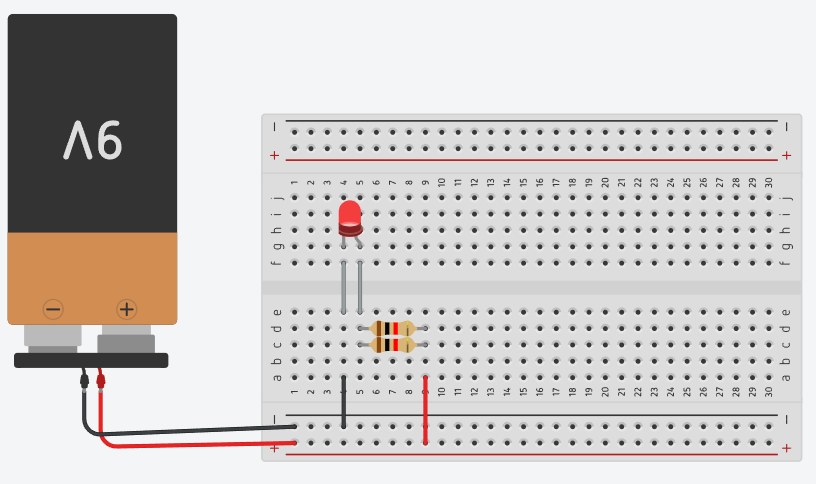
\includegraphics[width=0.5\textwidth]{./img/ckpt_2_2.png}
    \caption{2 Resistencia en paralelo}
    \label{fig:resistencia_paralelo}
\end{figure}

Ambos diodos LED se encienden, ya que las resistencias no limitan suficientemente la corriente que fluye a través de ellos. No obstante, el LED mostrado en la Figura \ref{fig:resistencia_serie} brilla con mayor intensidad en comparación con el de la Figura \ref{fig:resistencia_paralelo}, especialmente si se incrementa el valor de las resistencias.

\subsubsection{Circuito 2}

\begin{figure}[H]
    \centering
    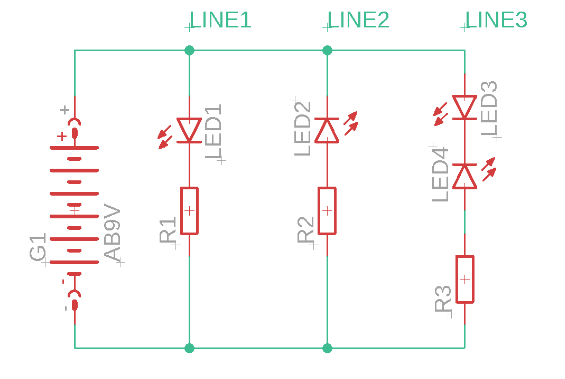
\includegraphics[width=0.5\textwidth]{./img/ckpt_2_3_0.png}
    \caption{Esquema de conexión}
    \label{fig:circuito_2}
\end{figure}

Se solicita simular (Figuras \ref{fig:simulacion_implementacion}, \ref{fig:simulacion_esquema1}) en Tinkercad el esquema presentado en la Figura \ref{fig:circuito_2} y responder las siguientes preguntas:

\begin{enumerate}
    \item \textbf{Descripción del circuito:} \\
    El circuito consiste en tres ramas conectadas en paralelo a una fuente de 9V. Cada rama contiene un LED en serie con una resistencia limitadora de corriente. Esto permite que cada LED tenga su propia ca\'ida de tensión y que la corriente se divida según la resistencia y caracter\'isticas del LED en cada l\'inea.

    \item \textbf{¿Qué sucede con el diodo LED en la L\'inea 1?} \\
    El LED en la L\'inea 1 enciende correctamente. La resistencia R1 limita la corriente, permitiendo que el LED funcione dentro de su rango seguro.

    \item \textbf{¿Qué sucede con el diodo LED en la L\'inea 2?} \\
    El LED en la L\'inea 2 no enciende. Esto se debe a que la polaridad del diodo est\'a invertida, lo que impide el paso de corriente. En este caso, la resistencia R2 no limita la corriente, ya que el LED no permite que fluya.

    \item \textbf{¿Qué sucede con el diodo LED en la L\'inea 3? ¿Por qué?} \\
    Ninguno de los LEDs en la L\'inea 3 enciende. Como ambos est\'an conectados en serie, la ca\'ida de tensión total requerida (~4.4V) puede superar la tensión disponible después de la resistencia R3. Adem\'as, dado que uno de los LEDs est\'a mal conectado (polaridad invertida), este interrumpe todo el paso de corriente en esa rama, impidiendo que cualquiera de los dos encienda.
\end{enumerate}

\begin{figure}[H]
    \centering
    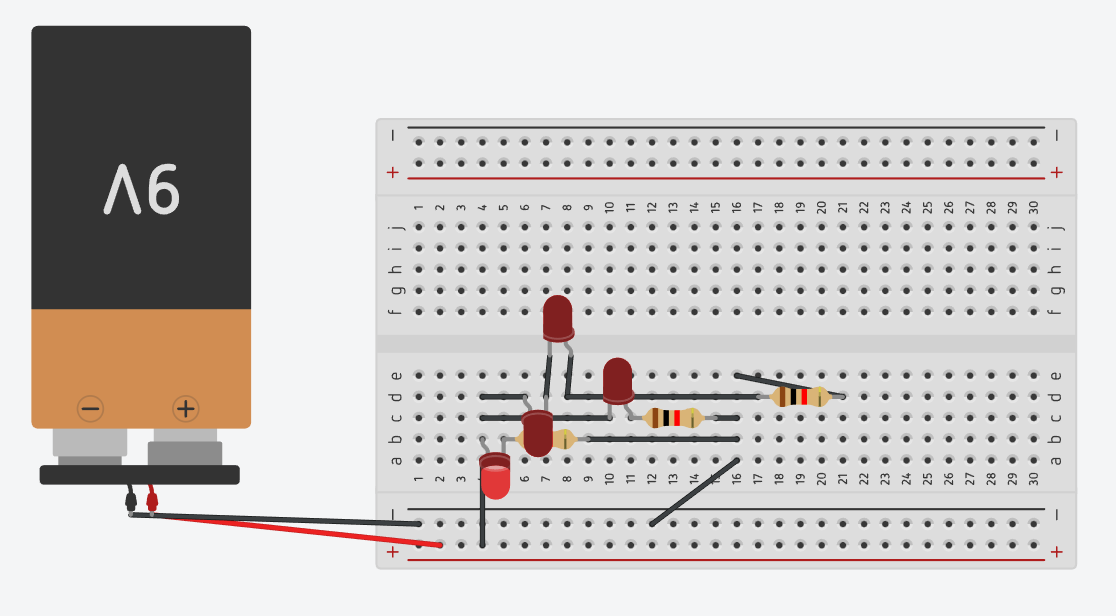
\includegraphics[width=0.85\textwidth]{./img/ckpt_2_3_1.png}
    \caption{Simulación Tinkercad del circuito.}
    \label{fig:simulacion_implementacion}
\end{figure}


\begin{figure}[H]
    \centering
    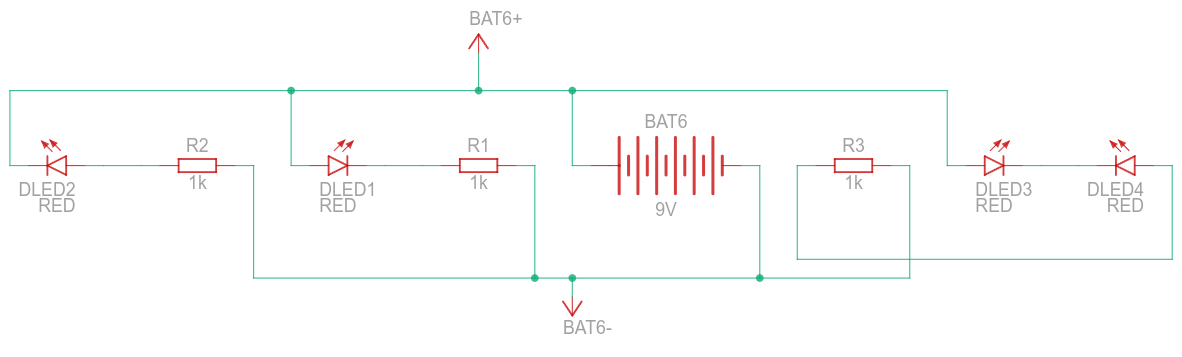
\includegraphics[width=0.85\textwidth]{./img/ckpt_2_3_2.png}
    \caption{Esquema de conexión Tinkercad}
    \label{fig:simulacion_esquema1}
\end{figure}

\subsection{Checkpoint 3: Simulación en FALSTAD}
Para el desarrollo de esta parte de la experiencia de laboratorio, nos hemos encargado de construir el siguiente circuito utilizando el programa \textbf{FALSTAD} para su simulación, como se muestra en la Figura \ref{fig:simulacion_esquema2}.

\begin{figure}[H]
    \centering
    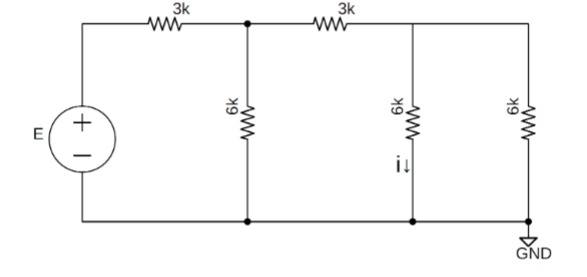
\includegraphics[width=0.85\textwidth]{./img/Circuito-3.jpeg}
    \caption{Circuito base}
    \label{fig:simulacion_esquema2}
\end{figure}

El circuito fue implementado en el simulador FALSTAD, como se observa en la Figura \ref{fig:simulacion_esquema3}, lo que permitió analizar su comportamiento y obtener los siguientes resultados:

\begin{figure}[H]
    \centering
    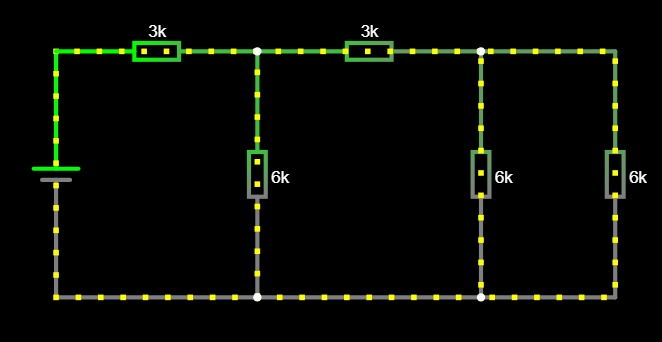
\includegraphics[width=0.85\textwidth]{./img/Falstad.jpeg}
    \caption{Circuito en simulador FALSTAD}
    \label{fig:simulacion_esquema3}
\end{figure}

Una vez realizada la simulación, hemos rescatado los siguientes datos:
\begin{itemize}
    \item El valor de la corriente ``i" es de 208.333 $\mu$A.
    \item La caída de tensión en la resistencia, siendo la última ubicada en la derecha, de 6k tiene un valor de 1.25 V.
    \item La potencia consumida por la fuente de alimentación tiene un valor de -4.167 mW.
\end{itemize}

\subsection{Checkpoint 4: LED con resistencia y potenciómetro}
En el siguiente experimento, hemos implementado el siguiente circuito, el cual nos permitirá conocer más a profundidad la función de un potenciómetro a través de los LEDs (Figura \ref{fig:simulacion_esquema4}).

\begin{figure}[H]
    \centering
    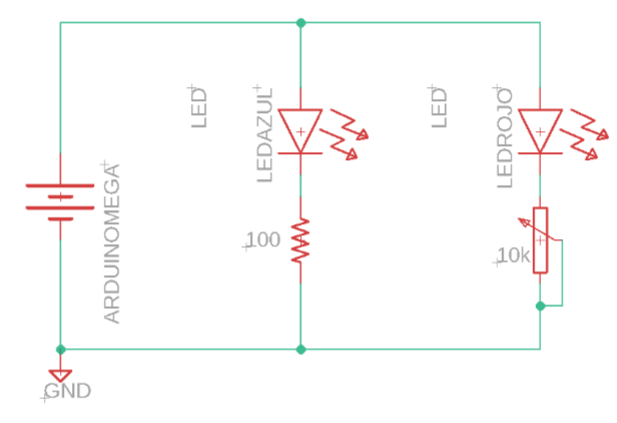
\includegraphics[width=0.50\textwidth]{./img/Circuito-potenciometro.png}
    \caption{Circuito base con potenciómetro}
    \label{fig:simulacion_esquema4}
\end{figure}

A través de la implementación pudimos entender su funcionamiento y determinar lo siguiente:
\begin{itemize}
    \item El LED azul estará siempre prendido una vez inicie el flujo de corriente, debido a que este se encuentra conectado, en serie, con una resistencia de 100 ohmios, permitiendo el flujo de corriente hacia tierra.
    \item El LED rojo también se encenderá si el pin del Arduino está en estado alto, sin embargo, su intensidad de brillo dependerá del valor ajustado en el potenciómetro de 10k ohmios.
    \item Al ajustar la perilla del potenciómetro se modifica la resistencia en el circuito, lo que cambia la cantidad de corriente que fluye a través del LED. Si disminuyes la resistencia, el LED rojo brillará con mayor intensidad porque circula más corriente; en cambio, si aumentas la resistencia, el brillo del LED disminuirá hasta apagarse si se llega al mínimo.
    \item Si la fuente de alimentación del Arduino la cambiamos de 5 a 3.3, ambos LEDs podrían verse afectados. En primer lugar, el LED azul no se enciende debido a que estos requieren un voltaje de mínimo 3V y si sumamos la resistencia se pierde mucha corriente ocasionando esto. Por otro lado, el LED rojo sí se sigue encendiendo pero con menor brillo, ya que hay menos voltaje y corriente disponibles, especialmente si el potenciómetro está ajustado a un valor alto.
\end{itemize}

La implementación del circuito se muestra en las Figuras \ref{fig:simulacion_esquema5} y \ref{fig:simulacion_esquema6}, donde se observa el comportamiento de los LEDs al variar el potenciómetro.

\begin{figure}[H]
    \centering
    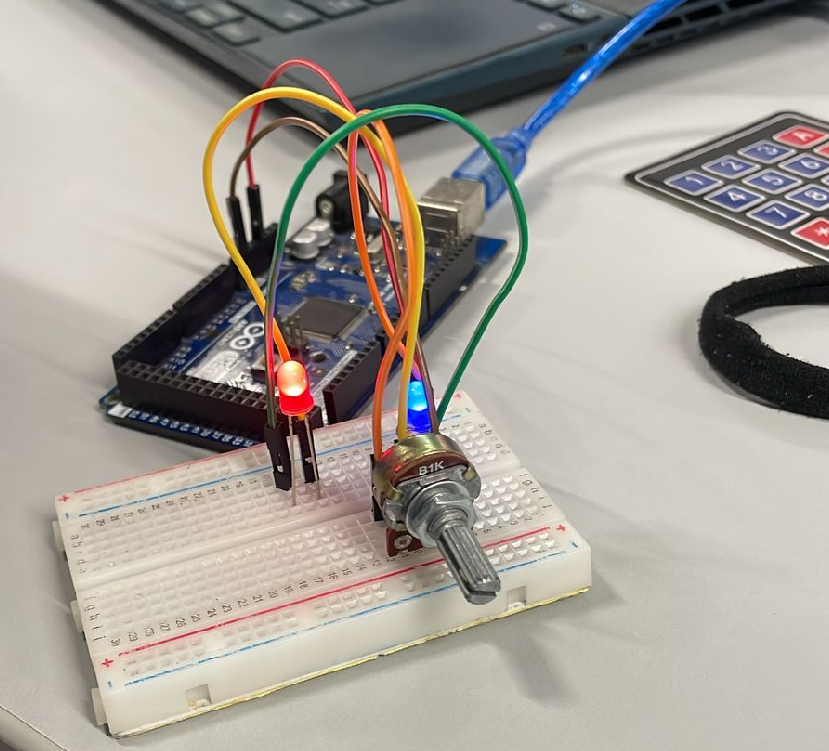
\includegraphics[width=0.50\textwidth]{./img/ckpt_3_4_2.png}
    \caption{Implementación LED-Potenciómetro (vista 1)}
    \label{fig:simulacion_esquema5}
\end{figure}

\begin{figure}[H]
    \centering
    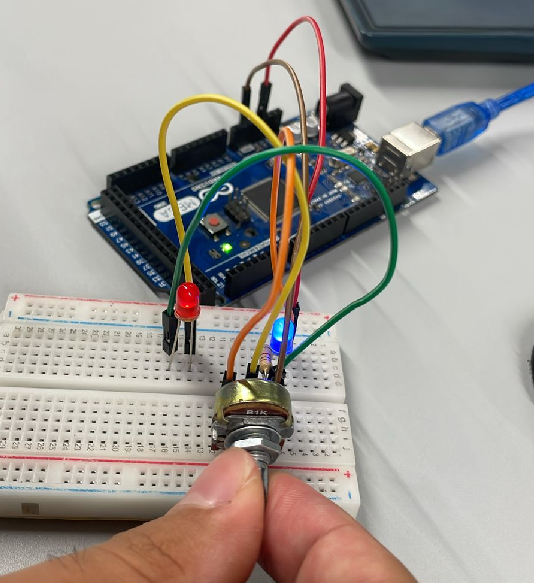
\includegraphics[width=0.50\textwidth]{./img/ckpt_3_4_1.png}
    \caption{Implementación LED-Potenciómetro (vista 2)}
    \label{fig:simulacion_esquema6}
\end{figure}

\subsection{Checkpoint 5: Uso de un botón}
En esta sección se explora el comportamiento de un circuito digital mediante el uso de un botón configurado como entrada, empleando una conexión tipo pull-up. Esta configuración es común en sistemas embebidos, ya que permite asegurar un estado lógico definido en ausencia de interacción física. En este caso, se busca controlar el encendido de un LED utilizando un botón conectado a tierra.

\begin{figure}[H]
    \centering
    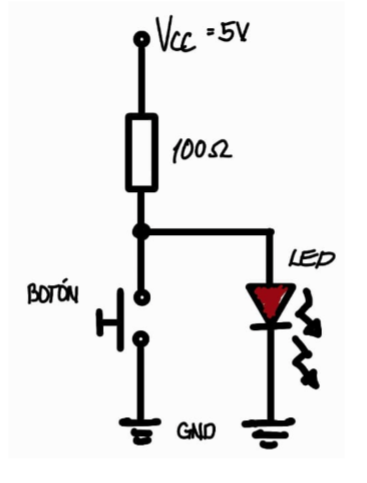
\includegraphics[width=0.50\textwidth]{./img/Circuito-boton.png}
    \caption{Circuito base con botón}
    \label{fig:simulacion_esquema7}
\end{figure}

El circuito se ha diseñado de tal manera que, por defecto, el LED permanece encendido, aprovechando que el voltaje en la salida es alto mientras el botón no es presionado. Al oprimir el botón, la salida se conecta a GND, lo que provoca que el voltaje caiga a nivel bajo y el LED se apague. Esta lógica de control resulta útil para ilustrar el funcionamiento de entradas digitales activas en bajo (active-low) y para analizar el efecto de cambiar la configuración a pull-down, lo cual invertiría completamente el comportamiento del sistema, es decir, por defecto estaría apagado y al presionar el botón el circuito se cerraría cambiando a prendido. La Figura \ref{fig:simulacion_esquema7} muestra el esquema a implementar y los resultados se muestran en la Figura \ref{fig:simulacion_esquema8}.

\begin{figure}[H]
    \centering
    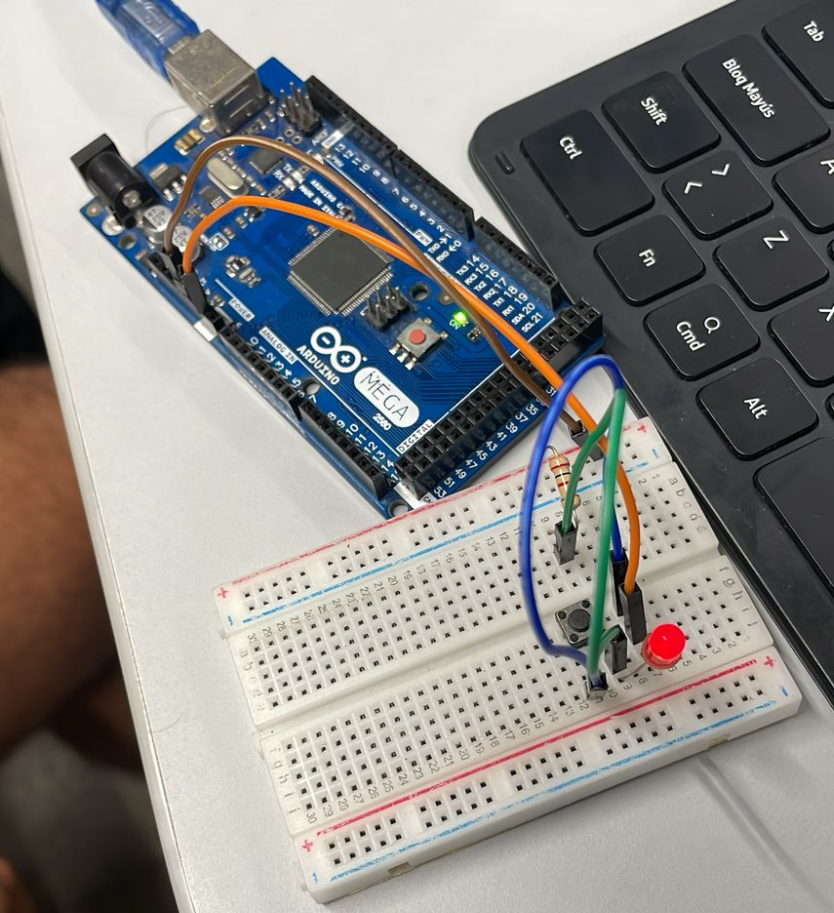
\includegraphics[width=0.50\textwidth]{./img/ckpt_3_5_1.png}
    \caption{Implementación del circuito con botón usando Arduino}
    \label{fig:simulacion_esquema8}
\end{figure}

\subsection{Checkpoint 6: LEDs secuenciales}

En este ejercicio se propone el dise\~no y simulación (Figura \ref{fig:leds_secuenciales}) de un sistema que utiliza cuatro diodos LED (rojo, azul, verde y amarillo) que se encienden de manera secuencial en un orden predefinido. Adem\'as, se incluye un botón que permite cambiar la dirección de la secuencia de encendido de los LEDs de forma instant\'anea, sin necesidad de completar el ciclo actual. Este sistema busca reforzar los conceptos b\'asicos de control de hardware mediante Arduino, incluyendo el uso de salidas digitales y la lectura de entradas digitales para modificar el comportamiento del sistema.

El funcionamiento del sistema se puede dividir en dos modos: 
\begin{itemize}
    \item \textbf{Modo normal (sin presionar el botón):} los LEDs se encienden en el orden rojo → azul → verde → amarillo.
    \item \textbf{Modo inverso (botón presionado):} los LEDs se encienden en el orden amarillo → verde → azul → rojo.
\end{itemize}

La transición entre modos se realiza al detectar un cambio en el estado del botón, y la dirección del encendido cambia de inmediato, lo cual se controla mediante una variable lógica \texttt{flag}.

\begin{figure}[H]
    \centering
    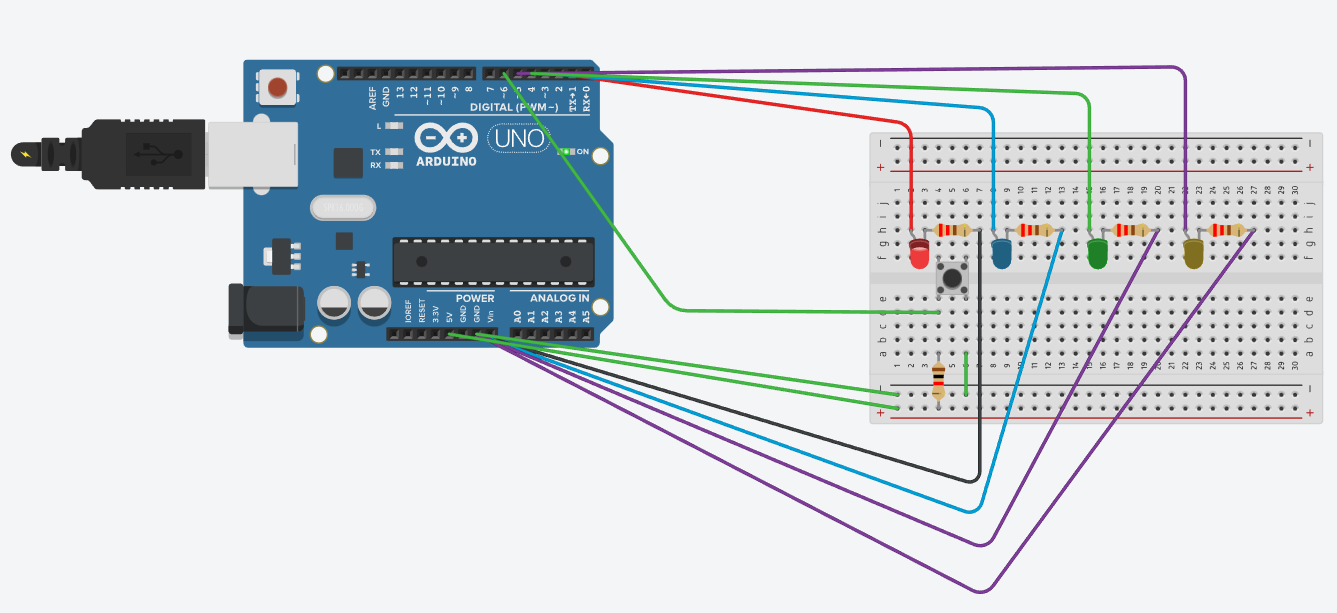
\includegraphics[width=0.85\textwidth]{./img/ckpt_6_0.png}
    \caption{Simulación Tinkercad LEDs secuenciales}
    \label{fig:leds_secuenciales}
\end{figure}

El código mostrado a continuación permite gestionar esta lógica. Cada vez que se ejecuta el bucle \texttt{loop()}, se verifica el estado del botón. Si est\'a presionado, se invierte la dirección de la secuencia. Luego, se incrementa la variable \texttt{color}, y se decide cu\'al LED encender según el valor de \texttt{color \% 4} y la dirección actual (\texttt{flag}). Al finalizar, se enciende el LED correspondiente durante un segundo y luego se apaga.


\begin{lstlisting}[style=cppstyle, caption={Código en C++ para el control de LEDs secuenciales.}, label={code:leds_secuenciales}]
// C++ code
int actual = 0, color = 0;
bool flag = 1;

void setup()
{
    pinMode(LED_BUILTIN, OUTPUT);
    pinMode(0, OUTPUT);
    pinMode(6, INPUT);
    pinMode(5, OUTPUT);
    pinMode(2, OUTPUT);
    pinMode(3, OUTPUT);
    pinMode(4, OUTPUT);
    Serial.begin(9600);
}

void loop()
{ 
    int buttonState = digitalRead(6);
    Serial.println(digitalRead(6));
    if (buttonState == LOW) flag = !flag;
    color += 1;
    if (flag)
    {
        if (color % 4 == 1) actual = 2;
        if (color % 4 == 2) actual = 3;
        if (color % 4 == 3) actual = 4;
        if (color % 4 == 0) actual = 5;
    } 
    else 
    {
        if (color % 4 == 1) actual = 5;
        if (color % 4 == 2) actual = 4;
        if (color % 4 == 3) actual = 3;
        if (color % 4 == 0) actual = 2;
    }
    digitalWrite(actual, HIGH);
    delay(1000);
    digitalWrite(actual, LOW);
}
\end{lstlisting}

Para facilitar la comprensión del algoritmo y su lógica de decisión, se elaboró el siguiente diagrama de flujo (Figura \ref{fig:leds_secuenciales_flowchart}). Este representa gr\'aficamente la secuencia de decisiones y acciones que se ejecutan en el ciclo principal del programa. En él se observa cómo se lee el estado del botón, se actualiza el contador y se determina el LED que debe encenderse, de acuerdo con la dirección actual.

\begin{figure}[H]
    \centering
    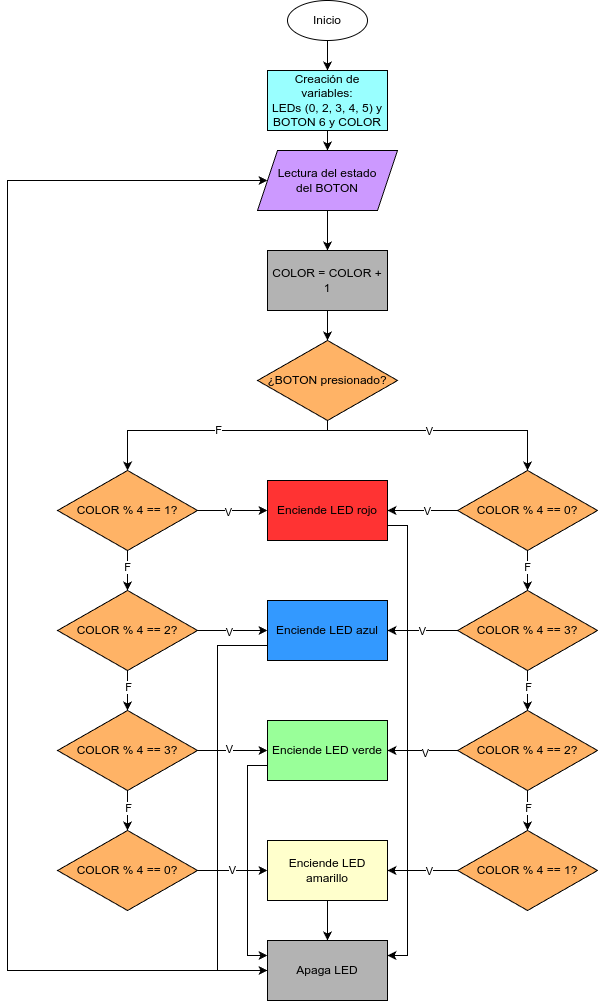
\includegraphics[width=0.6\textwidth]{./img/ckpt_6_1.png}
    \caption{Simulación Tinkercad LEDs secuenciales}
    \label{fig:leds_secuenciales_flowchart}
\end{figure}

\subsection{Checkpoint 7: Sem\'aforo}

Este ejercicio propone el diseño, simulación (Figura \ref{fig:simulacion_semaforo}) y la implementación de un sistema de semáforo (Figura \ref{fig:implementacion_semaforo}), simulando el comportamiento real de un cruce vehicular y peatonal. El objetivo es comprender cómo gestionar múltiples salidas digitales mediante temporización, estableciendo una lógica secuencial con distintos tiempos de activación. Para ello, se controlan dos sistemas simultáneos: un semáforo de vehículos con tres estados (rojo, verde y amarillo), y un semáforo peatonal con dos estados (caminar y detenerse).

A continuación el diagrama de flujo (Figura \ref{fig:flujo_semaforo}) que se diseño para representar el código a implementar.

\begin{figure}[H]
    \centering
    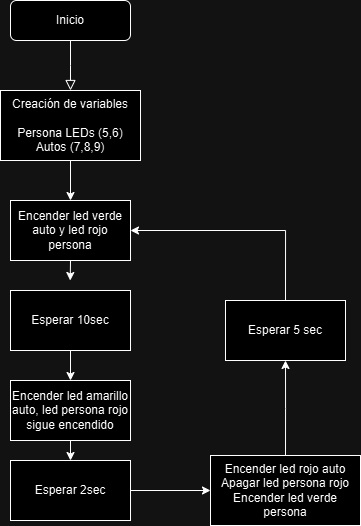
\includegraphics[width=0.6\textwidth]{./img/flujo_semaforo.png}
    \caption{Diagrama de flujo}
    \label{fig:flujo_semaforo}
\end{figure}

La lógica del sistema se basa en tiempos de permanencia predeterminados para cada luz (rojo: 10 segundos, verde: 5 segundos, amarillo: 2 segundos), lo que permite replicar el comportamiento típico de una intersección vial.

\begin{figure}[H]
    \centering
    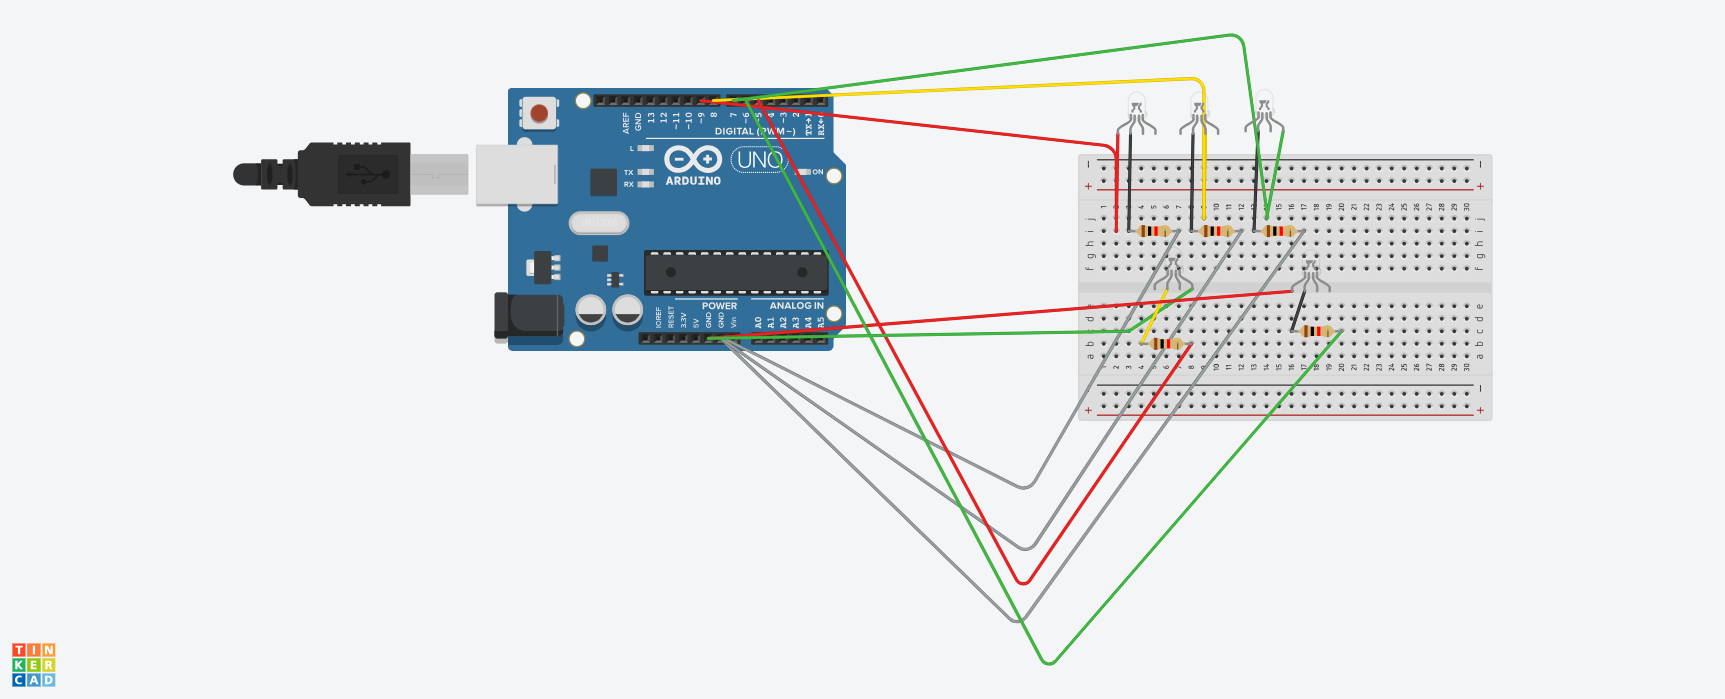
\includegraphics[width=0.9\textwidth]{./img/simulacion_semaforo.png}
    \caption{Simulación Tinkercad semáforo}
    \label{fig:simulacion_semaforo}
\end{figure}

\begin{figure}[H]
    \centering
    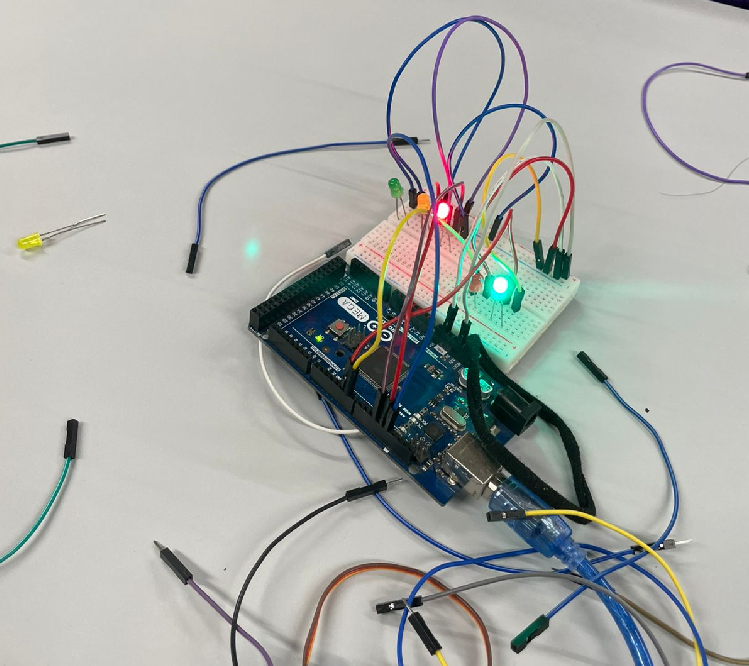
\includegraphics[width=0.6\textwidth]{./img/semaforo.png}
    \caption{Implementación semáforo}
    \label{fig:implementacion_semaforo}
\end{figure}

\section{Conclusiones}

A lo largo del desarrollo del Laboratorio 1 se logró reforzar la comprensión de los principios básicos de la electrónica y su aplicación directa mediante la plataforma Arduino. La implementación de circuitos físicos y su correspondiente simulación permitieron identificar el comportamiento real de componentes como LEDs, resistencias, potenciómetros y pulsadores, y cómo estos interactúan con señales digitales. El uso de simuladores como Tinkercad y Falstad facilitó el análisis sin riesgos y permitió detectar errores conceptuales antes de realizar montajes reales. Asimismo, el desarrollo de lógica de control a través de diagramas de flujo y programación en C/C++ fortaleció habilidades fundamentales en sistemas electrónicos. Finalmente, esta experiencia sirvió como punto de partida para enfrentar retos más complejos en el diseño de sistemas electrónicos interactivos, sentando las bases para una formación práctica sólida y contextualizada.


\bibliographystyle{plain}
\bibliography{bibliografia}

\end{document}

% https://tug.ctan.org/info/undergradmath/undergradmath.pdf
